\documentclass{article}
\usepackage[utf8]{inputenc}

\title{TKG Automation with Cloud Assembly}
\author{Tim Gretler}
\date{May 2020}

\usepackage{natbib}
\usepackage{graphicx}

\begin{document}



\maketitle


\newpage
\tableofcontents
\newpage


\section{Introduction}
This is a Guide on how to automate Tanzu Kubernetes Grid with Cloud Assembly and integrate it with Tanzu Mission Control, which are part of the VMware modern application portfolio \citep{tanzu}. It is thought to be a proof of concept to show how you can automate the control plane creation of Tanzu Kubernetes Grid. This will give you the ability to deploy a TKG management plane with a few clicks on AWS and vSphere. 

\subsection{Tanzu Kubernetes Grid}
Tanzu Kuberenetes Grid is certified Kubernetes distribution developed by VMware \citep{tkg}. It strives to build a simplified infrastructure across a multi-cloud environment. This will improve ease of development and also the speed of development, while still providing production grade stability. New automation capabilities provide a much faster and easier setup and therefore a higher flexibility in a diverse working environment. 

\subsection{Cloud Assembly}
Cloud Assembly is a VMware automation product \citep{cloudassembly}. It gives you a simple interface to your multi-cloud environment. With Cloud Assembly you have Infrastructure-as-Code and you are able to deploy templates to multiple cloud from a single interface. This provides the benefit of single source of truth for your deployments independent of the underlying cloud. 


\subsection{Tanzu Mission Control}
Tanzu Mission Control is the central control hub for your Kubernetes clusters \citep{tmc}. Tanzu Mission Control gives you insights to your fleet of clusters. One can also apply policies across all clusters from Tanzu Mission Control. You can attach any CNCF certified cluster and manage its lifecycle.

\newpage

\section{Manual}
\subsection{Prerequisites}
\begin{itemize}
  \item Access to Cloud Assembly
  \item vSphere Environment 
  \item AWS Account
\end{itemize}


\section{Troubleshooting}
``I always thought something was fundamentally wrong with the universe'' \citep{adams1995hitchhiker}


\begin{figure}[h!]
\centering
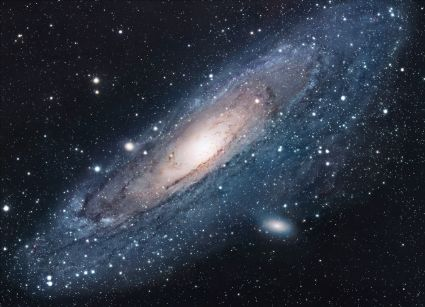
\includegraphics[scale=1.7]{universe}
\caption{The Universe}
\label{fig:universe}
\end{figure}


\bibliographystyle{plain}
\bibliography{references}
\end{document}
